\documentclass{llncs}
\usepackage{amsmath,amsfonts,amssymb}
\usepackage{graphicx}
\usepackage{makeidx}  % allows for indexgeneration
\begin{document}

\title{Simulation of Tsunami impact upon Coastline}

\titlerunning{Tsunami simulation}

\author{Aristotelis Spathis-Papadiotis\inst{1} \and Konstantinos Moustakas\inst{1}}
\authorrunning{Aristotelis Spathis-Papadiotis et al.} % abbreviated author list (for running head)

%%%% list of authors for the TOC (use if author list has to be modified)
\tocauthor{Konstantinos Moustakas, Aristotelis Spathis-Papadiotis}

\institute{Electrical and Computer Engineering Department\\
  University of Patras, Patra, Greece\\
  \email{moustakas@upatras.gr}}

\maketitle

\begin{abstract}
  This paper presents a simulation of a tsunami impact upon an urban coastline. Emphasis
  was given to the conservation of momentum, as its distribution in space and time is the
  main factor of the wave's effects on the coastline. Due to this, a hybrid simulation
  method was adopted, based on the Smoothed Particle Hydrodynamics (SPH) method, enriched
  with geometric constraints and rigid body interactions. The implementation is the result
  of cooperation between the Bullet physics engine and our custom SPH engine, which
  successively process the dynamic state of the fluid at every timestep. Furthermore, in
  order to achieve better performance a custom data structure (LP grid) was developed for
  the optimization of locality in data storage and minimization of access time. Simulation
  data is exported to VTK files, allowing interactive processing and
  visualization. Experimental results demonstrate the benefits of impulse recording at
  potential hazard estimation and evaluation of defense strategies. \keywords{Fluid
    simulation, tsunami, SPH, tsunami-coastline interaction, force visualization}
\end{abstract}

\section{Introduction}
Simulations of natural phenomena are a precious tool for analysis and understanding of the
processes behind them as well as the implications of those. Especially fluid dynamics is
one of the fields most benefitted by the explosion of high performance parallel computing
architectures of the last years. Tsunamis are one of the most devastating natural
disasters, with much attention drawn to them lately, especially after the 2004 Indian
Ocean tsunami and the 2011 T\={o}hoku earthquake and tsunami, two of the largest incidents
of modern history. Multiscale modelling of tsunami generation, propagation and impact is a
trending research area as respective simulations give valuable insights into the
underlying mechanisms and relations between the various stages of an unfolding tsunami
incident, while also facilitating the assessment of potential hazard it poses upon impact
on a coastline.

A tsunami is a series of waves in a water body caused by an impulsive disturbance that
vertically displaces a large volume of water. Tsunamis are generated by earthquakes,
volcanic eruptions, landslides and other such events which have the potential to transmit
a huge amount of mechanical energy to a water column. At large scales, tsunami propagation
in the ocean is usually modelled through various versions of the Shallow Water Equations,
derived from the Navier-Stokes equations in the case where the horizontal length scale is
much greater than the vertical one. Conversely, simulations of tsunami impact is usually
carried out using other methods, since complex dynamics must be taken into account. One of
the most used methods for simulating complex flows with multiple boundary interactions is
Smoothed Particle Hydrodynamics, initially proposed in the 1970s for the treatment of
compressible flows in astrophysical problems. Since then, it has been applied to a wide
variety of fields such as aerodynamics, geology, computer graphics and engineering with
exceptional results. In our simulation, emphasis was given to the conservation of momentum
and its distribution upon the coastline during the tsunami impact. Therefore, we adopted
SPH as our method of choice due to the unparalleled advantages it offers, relating to its
properties as lagrangian method.

\section{Related Work}
Computational fluid dynamics is a very active area of research, as it relates to a wide
spectrum of applications in computer graphics, engineering and science. The SPH method was
developed independently by Gingold and Monaghan \cite{gingold1977375} and Lucy
\cite{lucy19771013} in 1977. Since then it has been employed in a wide variety of problems
and applications, proving itself to be a flexible and attractive method for the simulation
of complex, multicomponent/multiphase flows. Its flexibility is shown by the numerous
adaptations and customizations it has undergone to suit many diverse problem domains.

Relating to the method itself, Desbrun and Gascuel \cite{desbrun1996smoothed} used it to
animate highly deformable bodies of various stiffness and viscosity, while proposing
important extensions like the ``spiky'' pressure smoothing kernel and discussing
implementation issues such as the surface reconstruction from density isosurfaces. Later,
M\"{u}ller et al. \cite{muller2003particle} used this work as a basis for fluid simulation
in interactive applications. Becker and Teschner \cite{becker2007weakly} developed Weakly
Compressible SPH, where the ideal gas equation of state is replaced with the much more
strict Tait equation to reduce compressibility to a user-defined upper bound, thus
avoiding an inefficient explicit Poisson equation solver. In recent years, Solenthaler and
Pajarola \cite{solenthaler2009predictive} improved WCSPH by proposing
Predictive-Corrective Incompressible SPH, where a prediction-correction scheme is used to
compute particle pressures through iterative density constraint satisfaction and
propagation through the fluid, until the final tolerance conditions are met. Implicit
Incompressible SPH was then proposed by Ihmsen et al. \cite{ihmsen2014implicit}, in which
the density is predicted using a discretized form of the pressure Poisson equation, as
obtained from the combination of a direct discretization of the continuity equation and
symmetric pressure forces.

Due to its adaptability and generality, SPH has been the method of choice for many
applications and relative extensions. Macklin and M\"{u}ller \cite{macklin2013position}
enriched SPH with positional geometric constraints, thus enforcing incompressibility while
maintaining stability and allowing for large timesteps. Rigid-fluid interaction is one of
the strong aspects of the method, as is shown by Akinci et al. \cite{akinci2012versatile},
where rigid surfaces are sampled by boundary particles, which adaptively contribute to
fluid properties to address boundary region deficiencies and inhomogeneities, in order to
incorporate rigid bodies to a unified hydrodynamic framework. Debroux et
al. \cite{debroux2001three} used SPH for the simulation of tsunami impact on real
coastline topography, where important features like the energy and speed of the wave were
measured over the course of time. Finally, a thorough overview of various implementation
algorithms and data structures together with their advantages and drawbacks is provided by
Dom\'{i}nguez et al. \cite{dominguez2011}.

\section{Proposed framework}
Our proposed simulation framework is based on SPH, a lagrangian fluid simulation method
whose core notion is the discretization of the fluid into particles, which serve as
interpolation points for the estimation of fluid properties in space. Advantages of this
method include the exact treatment of advection, the natural way of dealing with special
interface interactions, the inherent conservation of significant quantities (mass,
momentum, energy) and the self-adaptivity of computational load to the fluid location and
state in the flow domain. To efficiently ensure compressibility in degenerate cases and
undersampled boundary regions while maintaining relatively large timesteps, SPH was
enhanced with explicit solving of geometric constraints between particles. These
constraints are solved by the Bullet physics engine, within which fluid particles are
represented as rigid bodies, while also being subject to SPH forces as computed at each
timestep of the simulation.

\subsection{SPH method}
Starting from the identity:
\begin{equation*}
  f(\vec{r}) = \int_Vf(\vec{x}) \delta(\vec{r} - \vec{x}) d\vec{x},
\end{equation*}
where $\delta(\vec{r})$ the Dirac delta function and $\vec{x} \in V$, one can obtain a
more general interpolation rule by substituting $\delta(\vec{r})$ with a smoothing kernel
$W(\vec{r}, h)$:
\begin{equation*}
  \label{eq:c-approx}
  f(\vec{r}) \approx \int_V f(\vec{x}) W(\vec{r}-\vec{x}, h) d\vec{x}
\end{equation*}
whose limit when $h\to0$ approaches the delta fucntion and is normalized to unity:
\begin{equation*}
  \label{eq:kernel-properties}
  \lim_{h\to0}W(\vec{r}, h) = \delta(\vec{r})\ \ \
  \text{and}\ \ \
  \int_VW(\vec{r}, h) d\vec{x} = 1
\end{equation*}
The smoothing radius $h$ serves as a cutoff radius in the smoothing process, as particles
beyond that distance have no contribution to the sum, i.e. $W(r,h) = 0$ when $r>h$. For
the discrete case, where $f$ is discretized to particles with density $\rho$ and mass $m$,
the weighting ratio $m/\rho$ can be used to construct a weighted sum interpolant for any
field $A$:
\begin{equation}
  \label{eq:d-approx}
  A(\vec{r}) = \sum_i \frac{m_i}{\rho_i} A(\vec{r}_i) W(\vec{r}-\vec{r}_i, h)
\end{equation}
which lies at the heart of SPH formulation. According to this, the gradient can be
computed by the following approximation:
\begin{equation}
  \label{eq:d-grad}
  \nabla A(\vec{r}) = \sum_i \frac{m_i}{\rho_i} A(\vec{r}_i) \nabla W(\vec{r} - \vec{r}_i, h)
\end{equation}
The obvious advantage of this is the exclusive dependence on the smoothing kernel
gradient, which can be precomputed for sensible kernel choices. However, this formula can
lead to unsymmetric pair forces, compromising the conservation of linear and angular
momentum of the system. To symmetrize these forces depending on gradients (like those
originating from pressure differences), we can use the product rule:
\begin{equation*}
  \label{eq:grad-identity}
  \nabla \left( \frac{P}{\rho} \right) =
  \frac{\nabla P}{\rho}-
  \frac{P}{\rho^2} \nabla \rho
  \hspace{10pt} \Leftrightarrow \hspace{10pt}
  \nabla P = \rho \left[ \frac{P}{\rho^2} \nabla \rho + \nabla \left( \frac{P}{\rho}
    \right) \right]
\end{equation*}
to obtain an alternative approximation of gradient
\begin{align}
  \label{eq:grad-est}
  \nabla P & = \rho \left[ \frac{P}{\rho^2} \sum_i \frac{m_i}{\rho_i} \rho \nabla
             W(\vec{r}-\vec{r}_i, h)
             +
             \sum_i \frac{m_i}{\rho_i} \frac{P_i}{\rho_i} \nabla W(\vec{r}-\vec{r}_i, h)
             \right] \nonumber \\
           & = \rho \sum_i m_i \left(\frac{P}{\rho^2} + \frac{P_i}{\rho_i^2} \right)
             \nabla W(\vec{r}-\vec{r}_i, h)
\end{align}
which is antisymmetric for all interacting particle pairs. Viscosity forces on the other
hand, are proportional to the laplacian of the velocity field:
\begin{equation}
  \label{eq:lapl-est}
  \nabla^2\vec{v} = \sum_i \frac{m_i}{\rho_i} (\vec{v}_i - \vec{v}) \nabla^2
  W(\vec{r}-\vec{r}_i, h)
\end{equation}
and are always antisymmetric, since they depend on velocity difference
$\vec{v}_i - \vec{v}$ between particles.  In each timestep of the simulation, the density
of all particles is first computed according to equation (\ref{eq:d-grad}), as it depends
only on the relative position of those. The pressure at each particle location is then
obtained from its respective density through an equation of state. Subsequently, the
pressure and viscosity forces are computed from the particle data and integrated back into
the position and velocity of the particles.

\subsection{Implementation}
Each simulation under our implementation consists of two elements, the coastline terrain
(static) and the tsunami wave (dynamic). For the simulation setup, terrain is imported
from a suitable 3D geometry definition file format, the initial conditions of the
impacting wave (position and velocity) are configured, and the desired discretization
resolution for the fluid is set. From these conditions, the terrain and fluid are
initialized, and key parameters are computed as subsequently described. Terrain geometry
is scaled by a user-supplied factor and docked to the origin of coordinates, while fluid
particles are initially placed into an Hexagonal Close-Packed lattice, to achieve the
densest possible packing and symmetry:
\begin{equation}
  \label{eq:hcp}
  [x, y, z] = \left[ 2i+[(j+k) \bmod 2], \sqrt{3}[j + \frac{1}{3} (k \bmod 2)],
    \frac{2\sqrt{6}}{3} k \right] r
\end{equation}
In this configuration, the smoothing radius $h$ is computed such that each particle has
approximately 50 neighbours (following the empirical rule established in the
literature). The timestep is determined according to the Courant-Friedrichs-Lewy
criterion:
\begin{equation}
  \label{eq:cfl}
  \delta t_{\text{CFL}} = C \frac {\delta x}{v_{\text{max}}},
\end{equation}
for values of Courant number $C\approx0.5$ with characteristic length $\delta x$ equal to
the effective particle radius and maximum velocity $v_{\text{max}}$ determined by the
maximum potential energy in the initial configuration. Following standard practice, we
used three different smoothing kernels for density, pressure gradient and velocity
laplacian computation:
\begin{equation}
  \label{eq:poly6}
  W_{\text{poly6}}(r, h) = \frac{315}{64 \pi h^9}
  \begin{cases}
    (h^2 - r^2)^3 & 0 \leq r \leq h\\
    0 & \text{otherwise}
  \end{cases}
\end{equation}
\begin{equation}
  \label{eq:spiky}
  W_{\text{spiky}}(r, h) = \frac{15}{\pi h^6}
  \begin{cases}
    (h - r)^3 & 0 \leq r \leq h\\
    0 & \text{otherwise}
  \end{cases}
\end{equation}
\begin{equation*}
  \label{eq:spiky-gradient}
  \nabla W_{\text{spiky}}(r, h) = \frac{-45}{\pi h^6} (h-r)^2
\end{equation*}
\begin{equation}
  \label{eq:viscosity}
  W_{\text{viscosity}}(r, h) = \frac{15}{2 \pi h^3}
  \begin{cases}
    - \frac{r^3}{2h^3} + \frac{r^2}{h^2} + \frac{h}{2r} - 1 & 0 \leq r \leq h\\
    0 & \text{otherwise},
  \end{cases}\\
\end{equation}
\begin{equation*}
  \label{eq:viscosity-laplacian}
  \nabla^2 W_{\text{viscosity}}(r, h) = \frac{45}{\pi h^6} (h-r)
\end{equation*}

For the computation of the pressure from the estimated fluid density, the ideal gas
equation of state is used:
\begin{equation}
  \label{eq:ideal-state}
  P = k(\rho - \rho_0),
\end{equation}
according to which the pressure is proportional to the difference of the current from the
rest density. The major problem with this equation of state are the compressibility issues
that have been shown to exist in simulations using it. A frequently proposed solution is
to replace the above with the Tait equation of state:
\begin{equation}
  \label{eq:tait-state}
  P = B \left( \left( \frac{\rho}{\rho_0} \right)^\gamma - 1 \right),
\end{equation}
where usually $\gamma=7$ and $B$ a proportionality constant controlling the tolerance to
density fluctuations. This equation is much more punishing on density fluctuations away
from the rest density, therefore requiring significantly smaller timesteps to ensure
stability. Here we follow a different approach, inspired by Position Based Dynamics, in
which particles are represented by spherical rigid bodies. The most important advantage of
this technique is the elegant handling of boundary, undersampled and degenerate fluid
regions that tend to arise very frequently in simulations of free flows. The adoption of
this approach allows to treat boundary collisions in a simple manner, while naturally
enforcing incompressibility near boundaries and free surfaces. In these regions,
estimators fail to describe the actual flow regime due to neighbour particle
shortage. This undersampling creates the need for correction procedures, usually involving
ghost/boundary particles, to avoid pressure instabilities, particle clustering and other
artifacts. On the contrary, no such method is necessary under our representation, where
degenerative cases are handled through geometric constraints thus selectively preventing
unreliable estimations from affecting the flow.

\begin{figure}
  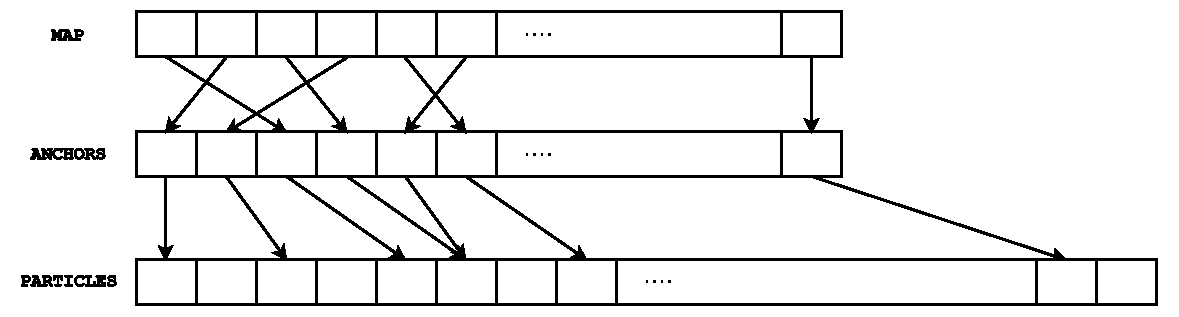
\includegraphics[width=\textwidth]{../report/figures/lp-grid.pdf}
  \caption{Organization of the custom data structure designed for the efficient storing
    and interaction scanning between simulation particles. Top-down, the first vector
    implements the 3D to linear locality preserving mapping of cell anchors onto the
    second, which in turn points to each cell's particles on the third.}
  \label{fig:lp-grid}
\end{figure}

The Bullet physics engine is used to handle the rigid body dynamics. The simulation domain
is divided by a regular grid of spacing equal to the smoothing radius into cells
containing the fluid particles, which are generated as Bullet objects and stored in a
custom cell list data structure consisting of three vectors. As shown in Figure
\ref{fig:lp-grid}, particles are accessed by following pointers through those vectors in
order, with the first encoding the 3D to linear locality preserving mapping of cells on
the second, and the second pointing at first of the cell's particles which are
continuously stored on the third, a dynamic sliding vector. This data structure allows for
quick neighbour search, interaction scanning, exploitation of access patterns of the SPH
algorithm and fast, in-place update. Simulation is following the Bullet framework, with
the SPH code being embedded as an internal timestep tick callback function. We took
advantage of the Bullet infrastructure to extract detailed information about the
collisions between fluid and terrain regarding the resulting impulse, time, and
location. Impulse and particle data are then written to multiple VTK files per
frame. Samples of the smoothed color field (common name in the literature for the field
having the value 1 at particle locations and 0 everywhere else) on the regular cell
lattice are also exported, which are then used to reconstruct the fluid surface as an
isosurface of that field. At the end of the simulation a cumulative impulse heatmap along
with the scaled and docked terrain model are also provided.

\section{Results}
Multiple simulations were carried out using different models of urban coastline, in order
to gain a significant and diverse dataset of impulses exerted over the duration of the
impact. Tsunamis are vastly different from the usual wind-induced sea waves in that they
have far longer wavelength and carry much greater total energy, appearing as a rapidly
rising tide instead of a breaking waves. Accounting for these facts, we chose to represent
the tsunami wave as a water volume invading the coastline with an initial velocity.

\begin{figure}[h!]
  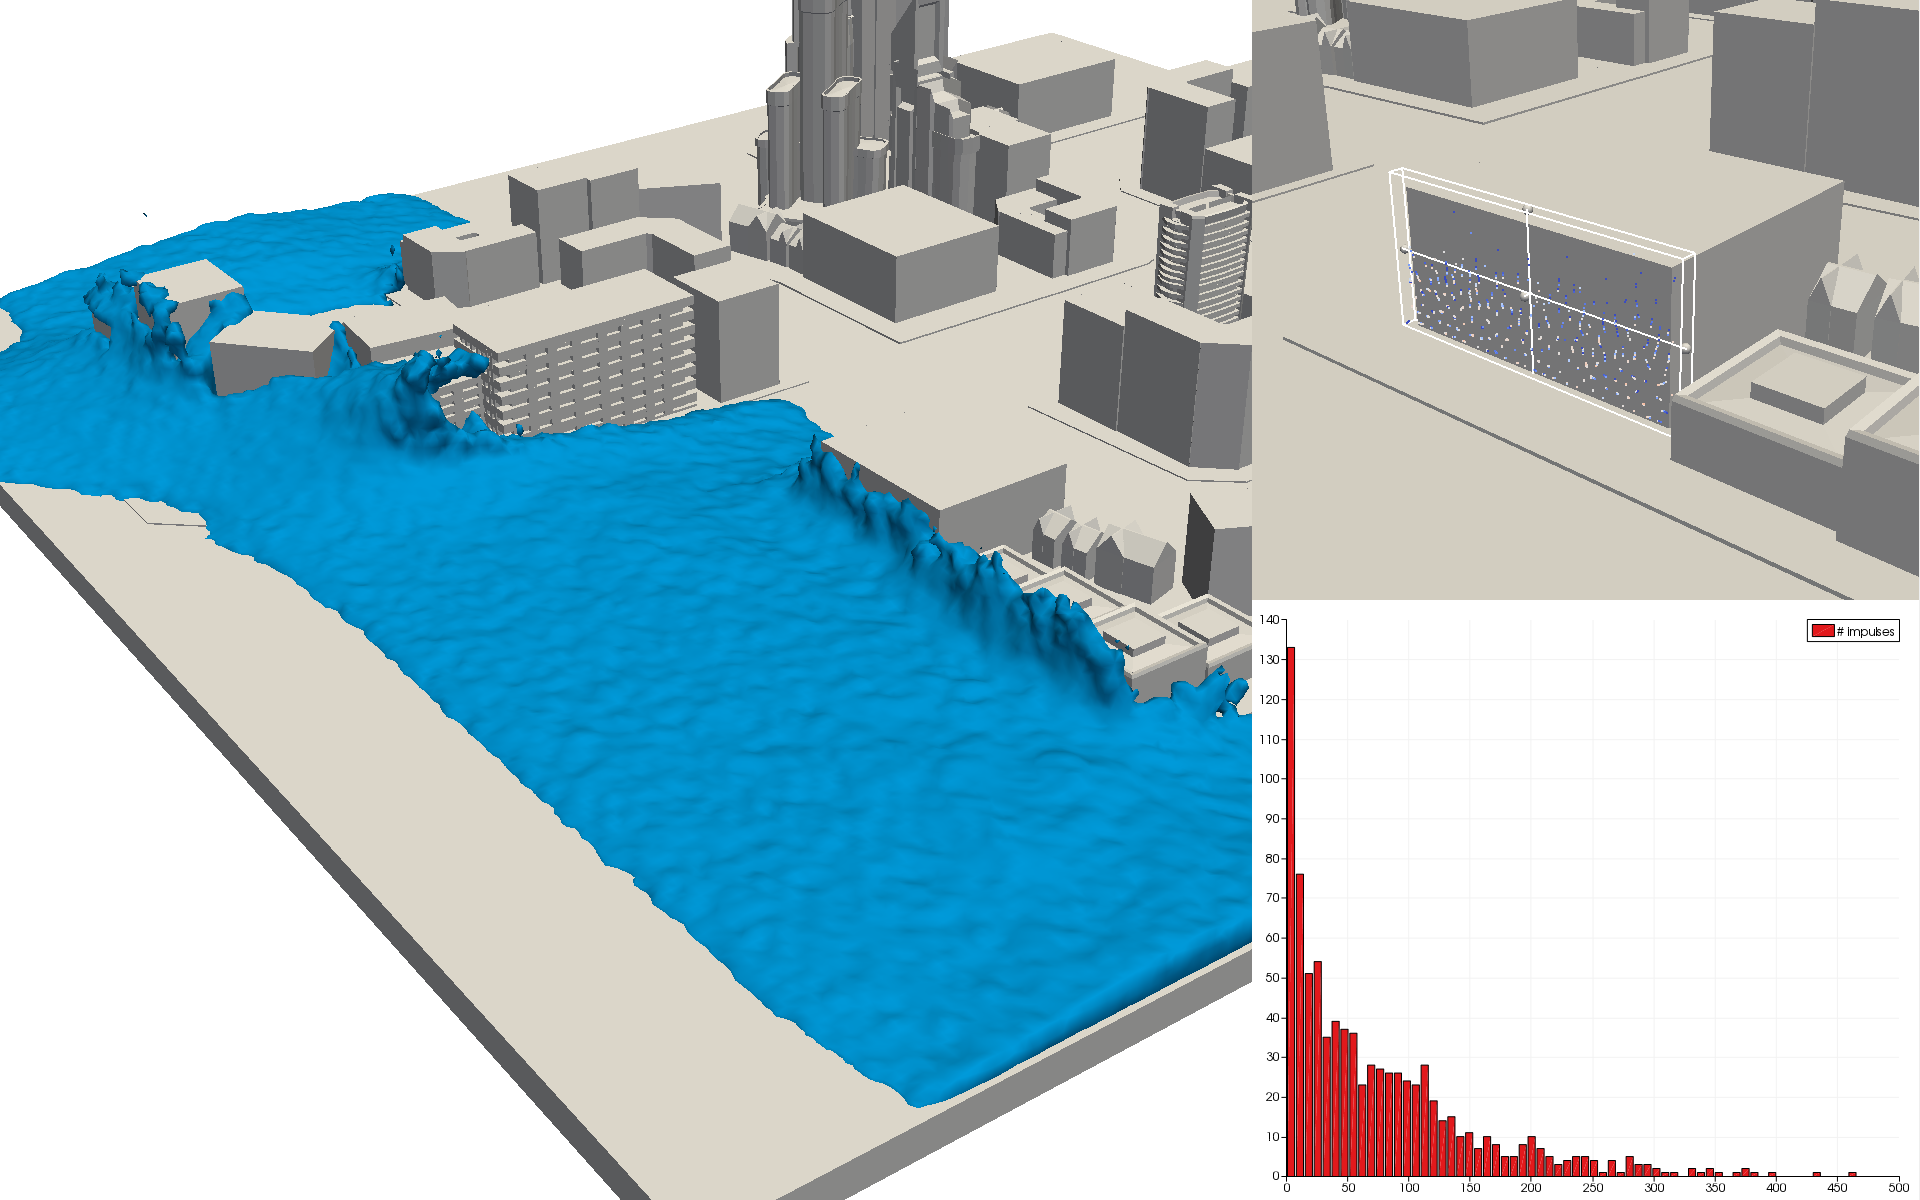
\includegraphics[width=\textwidth]{figures/paraview.png}
  \caption{Example visualization of impact data in Paraview\textsuperscript{TM}. Fluid
    surface is reconstructed as isosurface of fluid density, while impulses on the
    selected region are vi\-su\-a\-li\-zed as points on the 3D terrain model and in a
    histogram grouped by their magnitude.}
  \label{fig:visualization}
\end{figure}

Figure \ref{fig:visualization} shows a typical simulation result with the aid of
Paraview\textsuperscript{TM}, where the reconstructed wave surface and impulses exerted on
a selected region are visualized along the 3D terrain model and plotted on a histogram. A
comparison of the resulting impulse heatmap from the same tsunami impact upon an exposed
model and one with a protective seawall is shown in Figure \ref{fig:impulse-field}. These
heatmaps confirm a well-documented observation in the literature, i.e. that tsunami energy
is absorbed mostly by the first obstacle in its way. This has been noted by Danielsen et
al. \cite{danielsen2005asian} and Kathiresan and Narayanasamy \cite{kathiresan2005601},
who both emphasized the protective role coastal vegetation (mangrove forests) played in
mitigating the impact effects of the 2004 Indian Ocean tsunami. The same conclusion has
been reached by Yanagisawa et al. \cite{yanagisawa200927} through theoretical
approximation of the phenomenon backed by relevant field data and measurements. Seawalls
have been constructed in high-risk regions as a common countermeasure against tsunami
hazards. Although the waves may be so large as to overtop such barriers, these cases are
somewhat rare, making seawalls an effective first line of defense.

\begin{figure}
  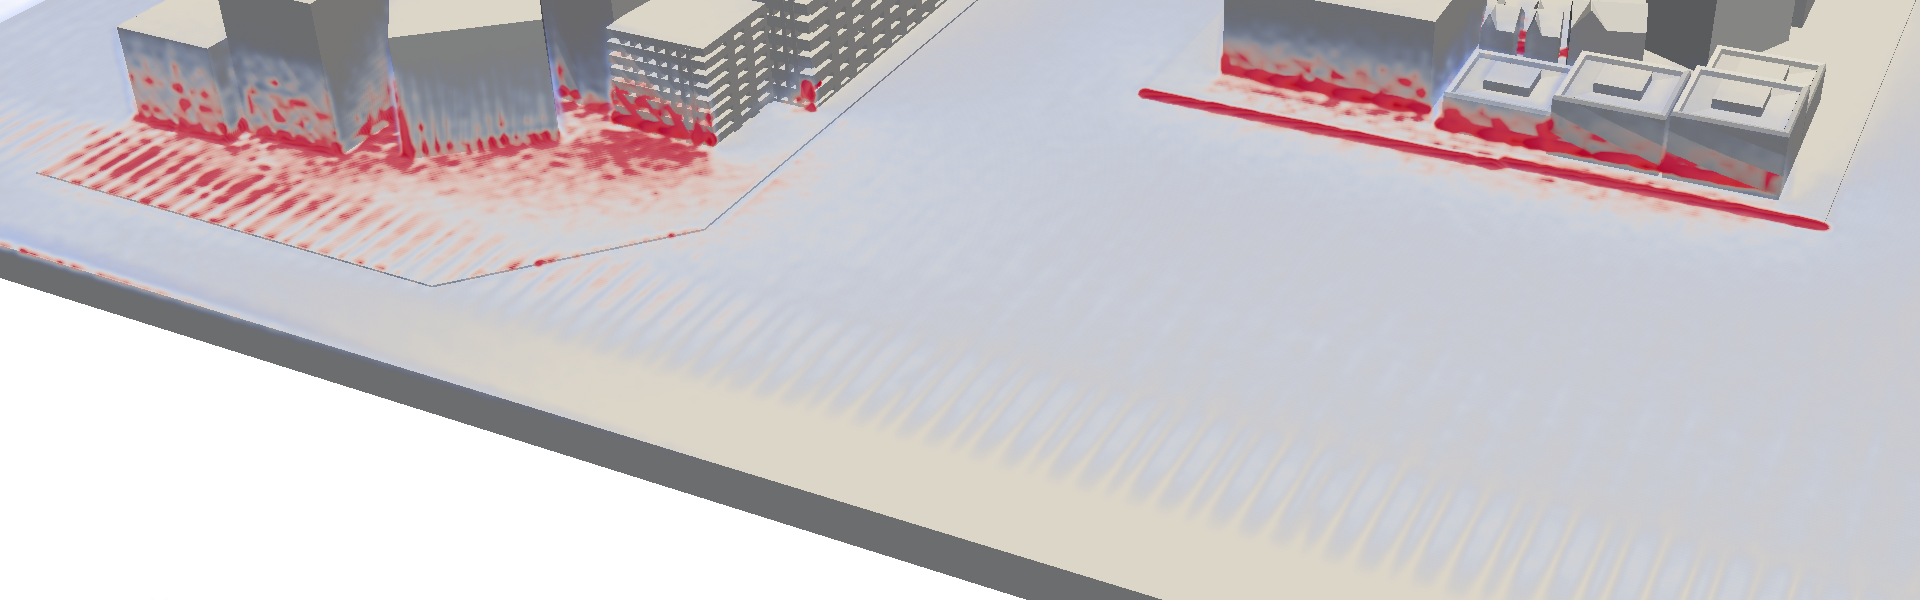
\includegraphics[width=\textwidth]{figures/if-city0-free.png}
  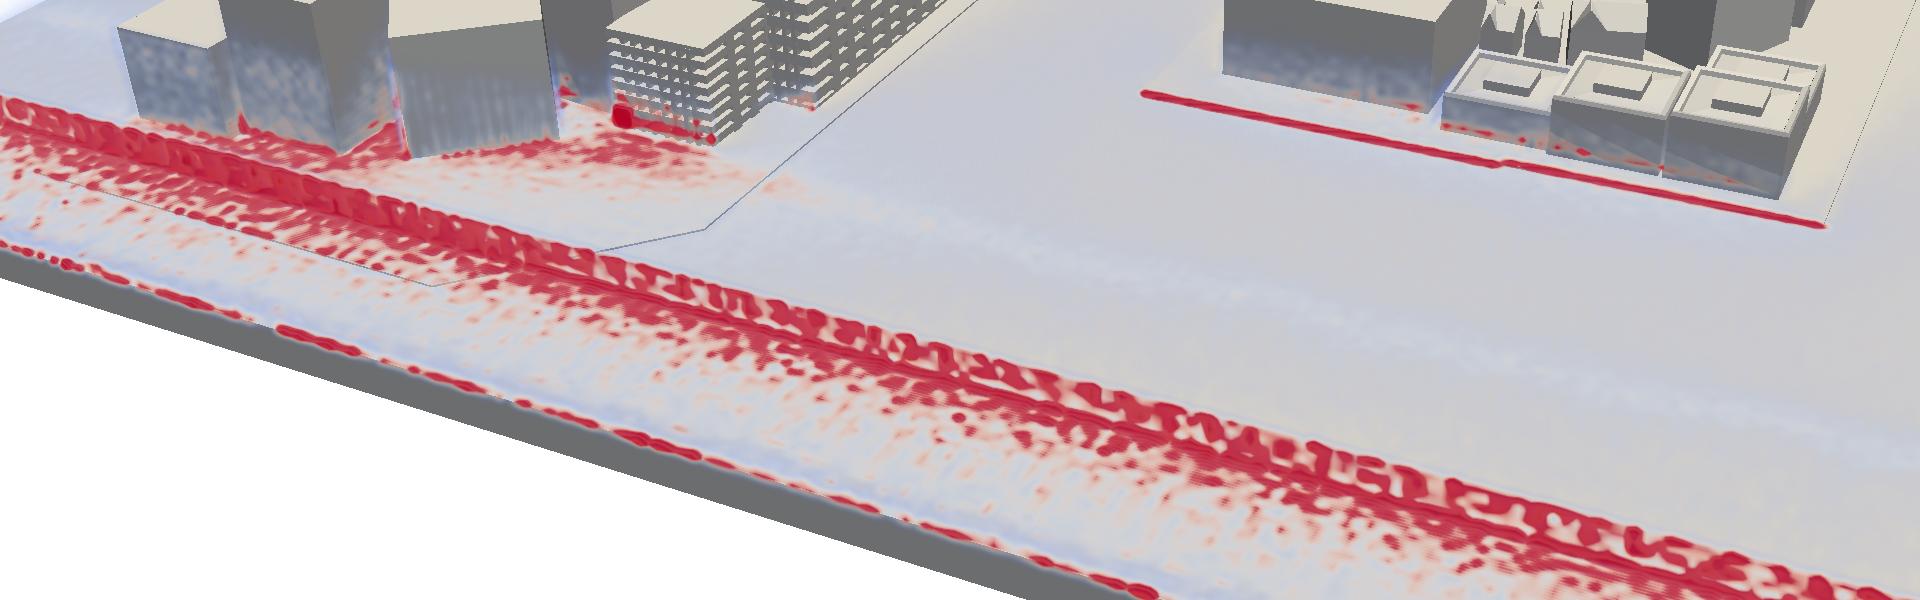
\includegraphics[width=\textwidth]{figures/if-city0-seawall.png}
  \caption{Comparison between the impulse heatmap of a tsunami hit on the same urban
    coastline model, with (up) and without (down) the protection from a seawall. Seawalls
    are commonly found in high-risk areas, as they reduce impact effects significantly.}
  \label{fig:impulse-field}
\end{figure}

The performance of the simulation program was satisfactory, there is however a substantial
margin for improvement. Figure \ref{fig:performance} shows a plot of the mean computation
time per output frame for variable fluid resolution. It is important to note that a higher
number of simulation particles imposes a shorter internal timestep due to their smaller
effective radius. These measurements are also representative of the worst-case scenario,
as due to the initial fluid conditions the particles are closely packed in a single body
of fluid, thus having maximum number of mutual interactions and reducing the performance
gains from our spatial hashing data structure. About 75\% of runtime is spent in
single-threaded code consisting mostly of Bullet and I/O operations and while the rest in
multi-threaded code of our SPH engine.

\begin{figure}
  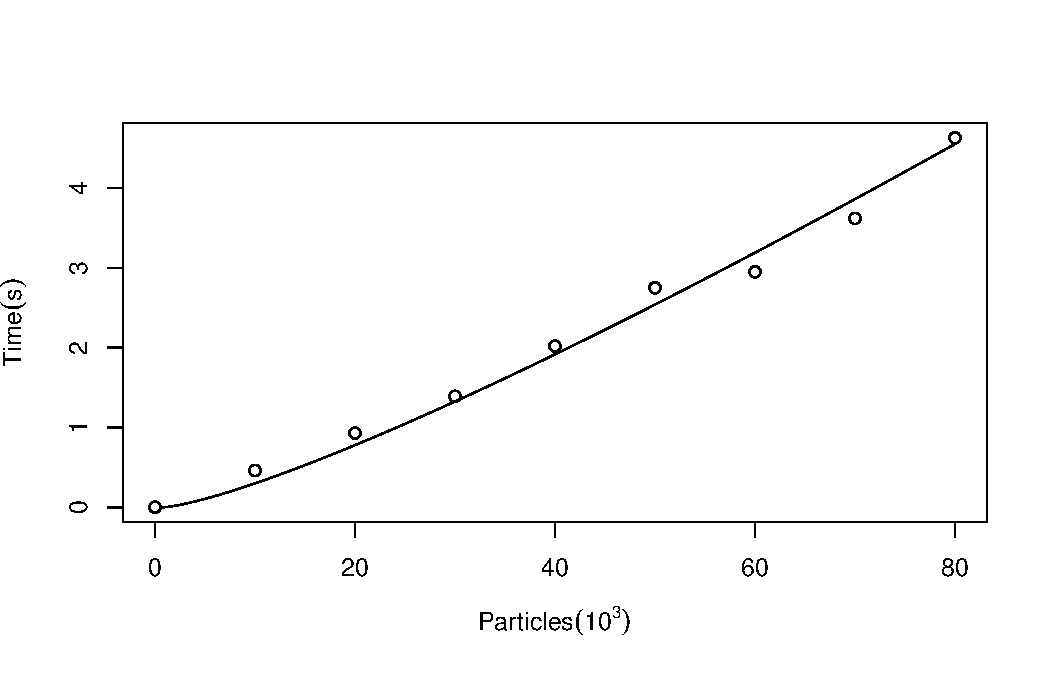
\includegraphics[width=\textwidth]{figures/performance.pdf}
  \caption{Plot showing the mean simulation time required per output frame for the
    simulation of the first 10 frames, for 10k to 80k particles (continuous line
    represents $O(n log_2n)$ growth).}
  \label{fig:performance}
\end{figure}

\section{Conclusions}
We presented the theoretical background and implementation of an enriched SPH framework,
whose main purpose was the faithful simulation and detailed recording of the forces
exerted upon the coastline during a tsunami impact. The chosen output file format lends
itself to rich visualizations, allowing for a quick overview of complex simulation
data. Multiple simulations have been carried out, resulting in interesting visualizations
of impact data and evaluation of defense mechanisms. Furthermore, detailed impulse logs
are provided, which can then be processed to extract relevant high level
information. Possible future extensions could be the incorporation of wider, dynamic
terrain models, including nearby seabed, the adjustment of the fluid initial conditions to
match those predicted by large-scale shallow water models, and performance optimizations
in the implementation towards a more integrated dataflow scheme.

% ---- Bibliography ----
\begin{thebibliography}{14}

\bibitem{akinci2012versatile} Akinci, N., Ihmsen, M., Akinci, G., Solenthaler, B.,
  Teschner, M.: Versatile rigid-fluid coupling for incompressible SPH. ACM Transactions on
  Graphics (TOG) 31(4), 62:1--62:8 (2012)

\bibitem{becker2007weakly} Becker, M., Teschner, M.: Weakly compressible SPH for free
  surface flows. In Proceedings of the 2007 ACM SIGGRAPH/Eurographics symposium on
  Computer animation, 209--217 (2007)

\bibitem{danielsen2005asian} Danielsen, F., S{\o}rensen, M. K., Olwig, M. F., Selvam, V.,
  Parish, F., Burgess, N. D., Hiraishi, T., Karunagaran, V. M., Rasmussen, M. S., Hansen,
  L. B. and Quarto, A.: The Asian tsunami: a protective role for coastal
  vegetation. Science(Washington) 310(5748), 643 (2005)

\bibitem{debroux2001three} Debroux, F., Prakash, M., Cleary, P.: Three-dimensional
  modelling of a tsunami interacting with real topographical coastline using Smoothed
  Particle Hydrodynamics. Proceedings of the 14th Australasian Fluid Mechanics Conference,
  Adelaide, Australia, 311--314 (2001)

\bibitem{desbrun1996smoothed} Desbrun M., Cani, M. P.: Smoothed particles: A new paradigm
  for animating highly deformable bodies. In Computer Animation and Simulation ’96
  (Proceedings of EG Workshop on Animation and Simulation), 61--76 (1996)

\bibitem{dominguez2011} Dom\'{i}nguez, J. M., Crespo, A. J., G\'{o}mez-‐Gesteira, M.,
  Marongiu, J. C.: Neighbour lists in smoothed particle hydrodynamics. International
  Journal for Numerical Methods in Fluids 67(12), 2026--2042 (2011)

\bibitem{gingold1977375} Gingold, R. A., Monaghan, J. J.: Smoothed particle hydrodynamics:
  theory and application to non-spherical stars. Monthly notices of the royal astronomical
  society 181(3), 375--389 (1977)

\bibitem{ihmsen2014implicit} Ihmsen, M., Cornelis, J., Solenthaler, B., Horvath, C.,
  Teschner, M.: Implicit incompressible SPH. Visualization and Computer Graphics, IEEE
  Transactions on 20(3), 426--435 (2014)

\bibitem{kathiresan2005601} Kathiresan, K., Rajendran, N.: Coastal mangrove forests
  mitigated tsunami. Estuarine, Coastal and Shelf Science 65(3), 601--606 (2005)

\bibitem{lucy19771013} Lucy, L. B.: A numerical approach to the testing of the fission
  hypothesis. The astronomical journal 82, 1013--1024 (1977)

\bibitem{macklin2013position} Macklin, M., M\"{u}ller, M.: Position Based Fluids. ACM
  Trans. Graph. 32(4), 104:1--104:12 (2013)

\bibitem{muller2003particle} M\"{u}ller, M., Charypar, D., Gross, M.: Particle-based fluid
  simulation for interactive applications. Proceedings of the 2003 ACM
  SIGGRAPH/Eurographics symposium on Computer animation, 154--159 (2003)

\bibitem{solenthaler2009predictive} Solenthaler, B., Pajarola, R.: Predictive-corrective
  incompressible SPH. In ACM transactions on graphics (TOG) 28(3) 40:1--40:6 (2009)

\bibitem{yanagisawa200927} Yanagisawa, H., Koshimura, S., Goto, K., Miyagi, T., Imamura,
  F., Ruangrassamee, A., Tanavud, C.: The reduction effects of mangrove forest on a
  tsunami based on field surveys at Pakarang Cape, Thailand and numerical
  analysis. Estuarine, Coastal and Shelf Science 81(1), 27--37 (2009)

\end{thebibliography}

\end{document}

%%% Local Variables:
%%% mode: latex
%%% TeX-master: t
%%% End:
